\begin{enumerate}[label=\thesection.\arabic*.,ref=\thesection.\theenumi]
\numberwithin{equation}{enumi}
\numberwithin{figure}{enumi}
\numberwithin{table}{enumi}
\item In figure,\figref{fig:rightangled4} BN and CM are medians of a $\triangle$ ABC right-angled at A. Prove that \begin{align}4(BN^2 +CM^2) = 5BC^2\end{align} 
\begin{figure}[!ht]
\centering
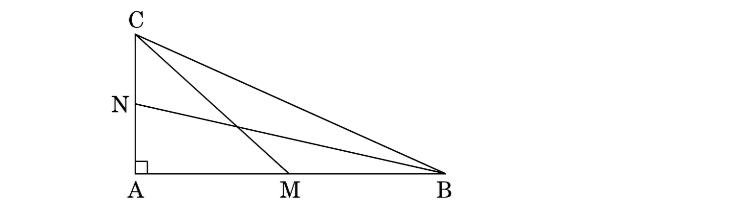
\includegraphics[width=\columnwidth]{figs/rightangled}
\caption{Right-angled triangle}
\label{fig:rightangled4}
\end{figure}
\item $\vec{Case Study - 1:}$
\begin{center}
$\vec{Kite Festival}$\\
\end{center}
Kite festival is celebrated in many countries at different times of the year. in India, every year 14th
January is celebrated as international kite Day. on his day many people visit India and participate in the festival by flying various kinds of kites.
\\The picture given below \figref{fig:kites5} , three kites flying together.
\begin{figure}[!ht]
\centering
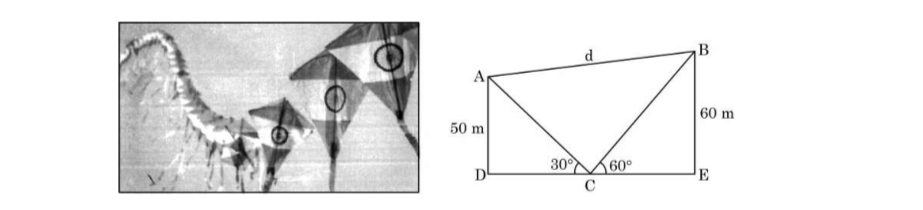
\includegraphics[width=\columnwidth]{figs/kites}
\caption{kites flying to gether}
\label{fig:kites5}
\end{figure}
\\In \figref{fig:kites5}, the angles of elevation of two kites (point C) are found to be $\degree{30}$ and  $\degree{60}$ respectively. Taking \begin{align}AD = 50 m\end{align} and\begin{align} BE = 60 m\end{align}
find 
\begin{enumerate}
\item The length of string used (take them straight) for kites A and B as shown in the figure.
\item The distance 'd' between these two kites
\end{enumerate}

\begin{enumerate}[label=\arabic*.,ref=\theenumi]
    \item In \figref{fig:fig1.png}, $PQ\parallel BC$, $PQ=3cm$, $BC=9cm$  and $AC=7.5cm$. Find the length of $AQ$.
    \begin{figure}[H]
        \centering
        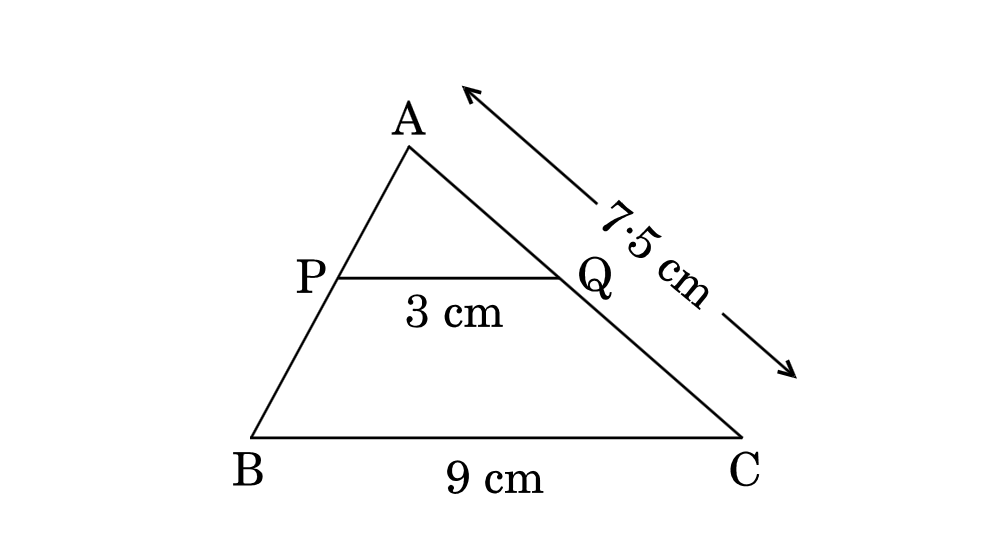
\includegraphics[width=\columnwidth]{./figs/figure1.png}
        \caption{$PQ\left |  \right | BC$}
        \label{fig:fig1.png}
    \end{figure}

    \item Draw a circle of radius $2.5cm$. Take a point $P$ outside the circle at a distance of $7cm$ from the centre. Then construct a pair of tangents to the circle from point $P$.

    \item Sides $AB$ and $AC$ and median $AD$ of $\triangle ABC$ are respectively proportional to sides $PQ$ and $PR$ and median $PM$ of $\triangle PQR$. Show that $\triangle ABC$  $\sim$  $\triangle PQR$.

     \item In \figref{fig:fig2.png} $BN$ and $CM$ are medians of a  $\triangle ABC$ right-angled at $A$. Prove that $4 (BN^2 + CM^2) = 5 BC^2$.

    \begin{figure}[H]
        \centering
        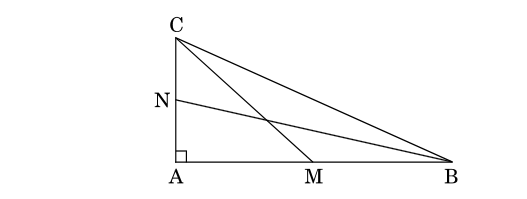
\includegraphics[width=\columnwidth]{./figs/figure2.png}
        \caption{ $BN$ and $CM$ are medians}
        \label{fig:fig2.png}
    \end{figure}

     \item Construct a pair of tangents to a circle of radius $4cm$ from a point $P$ lying outside the circle at a distance of $6cm$ from the centre.

     \item     

     \begin{enumerate}[label=(\alph*)]

     \item Draw a line segment $AB$ of length $8cm$ and locate a point $P$ 
      on $AB$ such that $AP$ : $PB$ = $1$ : $5$.

      \item  Draw a circle of radius $3 cm$. From a point $P$ lying outside the 
       circle at a distance of $6cm$ from its centre, construct two tangents
       $PA$ and $PB$ to the circle.

       \end{enumerate}

       \item Construct a pair of tangents to a circle of radius $5cm$ which are inclined each other at an angle of $60^{o}$.


        \item Write the steps of construction for constructing a pair of
         tangents to a circle of radius $4cm$ from a point $P$, at a distance
         of $7cm$ from its centre $O$.
\end{enumerate}
\end{enumerate}
	
